\documentclass[tikz]{standalone}
\usepackage{xcolor}
\newcommand\gry[1]{\definecolor{gry}{RGB}{#1,#1,#1}}
\begin{document}
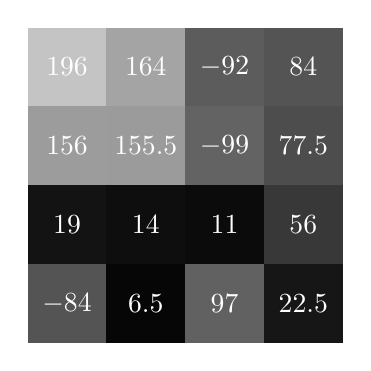
\begin{tikzpicture}
  \gry{196}\def\n{196}
  \path[fill=gry] (0,0) rectangle node[color=white]{$\n$} ++(1,-1);
  \gry{164}\def\n{164}
  \fill[gry] (1,0) rectangle node[color=white]{$\n$} ++(1,-1);
  \gry{92}\def\n{-92}
  \fill[gry] (2,0) rectangle node[color=white]{$\n$} ++(1,-1);
  \gry{84}\def\n{84}
  \fill[gry] (3,0) rectangle node[color=white]{$\n$} ++(1,-1);
  \gry{156}\def\n{156}
  \fill[gry] (0,-1) rectangle node[color=white]{$\n$} ++(1,-1);
  \gry{155}\def\n{155.5}
  \fill[gry] (1,-1) rectangle node[color=white]{$\n$} ++(1,-1);
  \gry{99}\def\n{-99}
  \fill[gry] (2,-1) rectangle node[color=white]{$\n$} ++(1,-1);
  \gry{77}\def\n{77.5}
  \fill[gry] (3,-1) rectangle node[color=white]{$\n$} ++(1,-1);
  \gry{19}\def\n{19}
  \fill[gry] (0,-2) rectangle node[color=white]{$\n$} ++(1,-1);
  \gry{14}\def\n{14}
  \fill[gry] (1,-2) rectangle node[color=white]{$\n$} ++(1,-1);
  \gry{11}\def\n{11}
  \fill[gry] (2,-2) rectangle node[color=white]{$\n$} ++(1,-1);
  \gry{56}\def\n{56}
  \fill[gry] (3,-2) rectangle node[color=white]{$\n$} ++(1,-1);
  \gry{84}\def\n{-84}
  \fill[gry] (0,-3) rectangle node[color=white]{$\n$} ++(1,-1);
  \gry{6}\def\n{6.5}
  \fill[gry] (1,-3) rectangle node[color=white]{$\n$} ++(1,-1);
  \gry{97}\def\n{97}
  \fill[gry] (2,-3) rectangle node[color=white]{$\n$} ++(1,-1);
  \gry{22}\def\n{22.5}
  \fill[gry] (3,-3) rectangle node[color=white]{$\n$} ++(1,-1);
\end{tikzpicture}
\end{document}